\documentclass[bachelor, och, coursework]{SCWorks}
% параметр - тип обучения - одно из значений:
%    spec     - специальность
%    bachelor - бакалавриат (по умолчанию)
%    master   - магистратура
% параметр - форма обучения - одно из значений:
%    och   - очное (по умолчанию)
%    zaoch - заочное
% параметр - тип работы - одно из значений:
%    referat    - реферат
%    coursework - курсовая работа (по умолчанию)
%    diploma    - дипломная работа
%    pract      - отчет по практике
% параметр - включение шрифта
%    times    - включение шрифта Times New Roman (если установлен)
%               по умолчанию выключен
\usepackage{subfigure}
\usepackage{tikz,pgfplots}
\pgfplotsset{compat=1.5}
\usepackage{float}

%\usepackage{titlesec}
\setcounter{secnumdepth}{4}
%\titleformat{\paragraph}
%{\normalfont\normalsize}{\theparagraph}{1em}{}
%\titlespacing*{\paragraph}
%{35.5pt}{3.25ex plus 1ex minus .2ex}{1.5ex plus .2ex}

\titleformat{\paragraph}[block]
{\hspace{1.25cm}\normalfont}
{\theparagraph}{1ex}{}
\titlespacing{\paragraph}
{0cm}{2ex plus 1ex minus .2ex}{.4ex plus.2ex}

% --------------------------------------------------------------------------%


\usepackage[T2A]{fontenc}
\usepackage[utf8]{inputenc}
\usepackage{graphicx}
\graphicspath{ {./images/} }
\usepackage{tempora}

\usepackage[sort,compress]{cite}
\usepackage{amsmath}
\usepackage{amssymb}
\usepackage{amsthm}
\usepackage{fancyvrb}
\usepackage{listings}
\usepackage{listingsutf8}
\usepackage{longtable}
\usepackage{array}
\usepackage[english,russian]{babel}

% \usepackage[colorlinks=true]{hyperref}
\usepackage{url}

\usepackage{underscore}
\usepackage{setspace}
\usepackage{indentfirst} 
\usepackage{mathtools}
\usepackage{amsfonts}
\usepackage{enumitem}
\usepackage{tikz}

\newcommand{\eqdef}{\stackrel {\rm def}{=}}
\newcommand{\specialcell}[2][c]{%
\begin{tabular}[#1]{@{}c@{}}#2\end{tabular}}

\renewcommand\theFancyVerbLine{\small\arabic{FancyVerbLine}}

\newtheorem{lem}{Лемма}

\begin{document}

% Кафедра (в родительном падеже)
\chair{теоретических основ компьютерной безопасности и криптографии}

% Тема работы
\title{Обнаружение объектов на изображении искусственными нейронными сетями}

% Курс
\course{2}

% Группа
\group{231}

% Факультет (в родительном падеже) (по умолчанию "факультета КНиИТ")
\department{факультета КНиИТ}

% Специальность/направление код - наименование
%\napravlenie{09.03.04 "--- Программная инженерия}
%\napravlenie{010500 "--- Математическое обеспечение и администрирование информационных систем}
%\napravlenie{230100 "--- Информатика и вычислительная техника}
%\napravlenie{231000 "--- Программная инженерия}
\napravlenie{100501 "--- Компьютерная безопасность}

% Для студентки. Для работы студента следующая команда не нужна.
% \studenttitle{Студентки}

% Фамилия, имя, отчество в родительном падеже
\author{Улитина Ивана Владимировича}

% Заведующий кафедрой
\chtitle{} % степень, звание
\chname{Абросимов М. Б.}

%Научный руководитель (для реферата преподаватель проверяющий работу)
\satitle{доцент} %должность, степень, звание
\saname{Слеповичев И. И.}

% Руководитель практики от организации (только для практики,
% для остальных типов работ не используется)
% \patitle{к.ф.-м.н.}
% \paname{С.~В.~Миронов}

% Семестр (только для практики, для остальных
% типов работ не используется)
%\term{8}

% Наименование практики (только для практики, для остальных
% типов работ не используется)
%\practtype{преддипломная}

% Продолжительность практики (количество недель) (только для практики,
% для остальных типов работ не используется)
%\duration{4}

% Даты начала и окончания практики (только для практики, для остальных
% типов работ не используется)
%\practStart{30.04.2019}
%\practFinish{27.05.2019}

% Год выполнения отчета
\date{2021}

\maketitle

% Включение нумерации рисунков, формул и таблиц по разделам
% (по умолчанию - нумерация сквозная)
% (допускается оба вида нумерации)
% \secNumbering

%-------------------------------------------------------------------------------------------

\tableofcontents

\intro

    В современном мире, в эпоху информационных технологий, с каждым годом увеличивается количество задач, которые могут быть решены с помощью компьютера. И чем сложнее компьютер становится, тем более серьезные проблемы становятся решаемыми. Однако были такие задачи, которые легко решались только человеческим разумом, а не вычислительной машиной, так как компьютером разрешались проблемы, имеющие математическую составляющую, то есть подход к которым осуществлялся с помощью определенного набора аксиом и правил. С момента появления компьютера, совсем недавно начала развиваться наука об искусственном интеллекте, которая открыла компьютерам возможность находить решения для таких проблем, которые раньше могли быть решены только человеком. Вследствие этого сейчас активно начала использоваться технология нейронных сетей, которая позволяет решать простые человеческие проблемы достаточно быстро, упрощая повседневную жизнь людей. 
    Вот несколько примеров задач, в которых используется искусственный интеллект:
    
    \begin{enumerate}
        \item Определение самого короткого маршрута из точки А в точку Б с учетом трафика в городе;
        \item Перевод с одного языка на другой;
        \item Автоматическое определение диагноза пациента при наборе симптомов;
        \item Парковка машины с помощью искусственного интеллекта;
        \item Сведение звука в музыкальных произведениях;
        \item Классификация большого объема данных каких-либо форматов по различным нетривиальным или неоднозначным ключам;
        \item Определение объектов на изображении;
        \item Формирование прогноза погоды на основе некоторой метеорологической базе данных;
        \item Предсказание курса ценных бумаг.
    \end{enumerate}

    В данной работе будет рассматриваться задача обнаружения объектов на изображении посредством искусственных нейронных сетей, её примеры в реальной жизни, математическая составляющая её решения и анализ соответствующих этому решению инструментов.

\defabbr

    Перед анализом математической составляющей нейронной сети, работающей с конкретной задачей (в данном случае "--- с анализом изображений на предмет обнаружения объектов) стоит ввести ряд терминов и определений, которые являются фундаментом понимания работы нейросетей.

    \textit{Граф} "--- абстрактное математическое понятие, определяющее объект, который состоит из совокупности вершин и рёбер, которые соединяют вершины.

    \textit{Сетевая топология} "--- вид графа, вершинами которого являются конечные узлы сети, а ребрами - связи между вершинами, содержащие информацию.

    \textit{Искусственный интеллект} (Artificial Intelligence) "--- технология создания алгоритмов, лежащих в основе проектирования интеллектуальных машин и программ, способных имитировать деятельность человека.

    \textit{Нейронная сеть (нейросеть)} (Neural Network) "--- математическая модель, чаще всего имеющая программную интерпретацию, сутью которой является реализация деятельности, похожей на деятельность биологических нейронных сетей. Нейронная сеть используется при создании какого-либо из алгоритмов искусственного интеллекта и состоит из совокупности нейронов, соединенных между собой связями. 

    \textit{Искусственный нейрон} "--- преобразователь одного или нескольких входных элементов в по крайней мере один выходной элемент в некоторый дискретный момент времени с определенным шагом.

    \textit{Входной, или видимый слой} (Input layer) "--- один нейрон или совокупность нейронов в нейросети, содержащая открытые, входные и неизмененные данные, которые включают в себя доступные для изучения переменные.

    \textit{Скрытый слой} (Hidden layer) "--- один нейрон или совокупность нейронов в нейросети, которая осуществляет вычисления и генерирует данные, не доступные для анализа и не являющиеся изначальными или конечными.

    \textit{Выходной слой} (Output layer) "--- один нейрон или совокупность нейронов в нейросети, представляющая собой результат работы нейронной сети.

    \textit{Признак} "--- каждый отдельный элемент информации, включаемый в представление о каком-либо анализируемом объекте.

    \textit{Машинное обучение} (Machine Learning) "--- область науки об искусственном интеллекте, которая изучает способы создания алгоритмов, которые могут обучаться (развиваться).

    \textit{Обучение представлений} "--- использование методов машинного обучения для определения представления.

    \textit{Автокодировщик} "--- совокупность функции кодирования (которая преобразует входные данные в удобное для решения задачи представление) и функции декодирования, являющейся обратной по смыслу к предыдущей функции.

    \textit{Фактор вариативности} "--- в контексте машинного обучения это концепция, помогающая получить смысл из данных той характеристики об изучаемом объекте, которая может иметь большое количество различных значений, то есть обладающая высокой вариативностью.

    \textit{Глубокое обучение} (Deep Learning) "--- частный случай машинного обучения, который представляет из себя методы машинного обучения, основанные на обучении представлений. Осуществляет получение представлений путем их выражения через более простые представления, а формирование последних, в свою очередь, реализуется через ещё более простые представления, и так далее.

    \textit{Компьютерное зрение} (Computer Vision) "--- область науки об искусственном интеллекте, использующая методы машинного и глубокого обучения для решения задач распознавания, классификации, мониторинга с помощью получения необходимой информации из изображения.

\section{Концепция технологии}

    \subsection{Математическая составляющая нейронной сети}
        Для понимания работы алгоритмов машинного обучения, которые активно применяются при реализации компьютерного зрения, следует иметь представления о нейронных сетях, которые эти алгоритмы используют.
        
        Структура нейронной сети представляет из себя результат деятельности нескольких математических дисциплин, среди которых следует выделить несколько важных для нас: 
            
            \begin{enumerate}
                \item Линейная алгебра "--- область математики, а именно раздел алгебры, который изучает объекты линейной природы: скаляры, векторы, матрицы, определители, сопряжения, линейные отображения, системы линейных уравнений, линейные и векторные пространства и т.д. Она используется во многих алгоритмах машинного и глубокого обучения.
                \item Теория вероятностей "--- область математики, в которой рассматриваются недостоверные утверждения, то есть события, которые могут произойти с определенным шансом на успех. Она определяет средства, с помощью которых можно количественно описать недостоверность событий, а также предоставляет аксиомы для вывода новых недостоверных суждений. Так как машинное обучение работает с стохастическими и неопределенными событиями, применение теории вероятностей необходимо.
                \item Теория графов "--- область математики, изучающая графы, а также связанные с ним понятия, операции и алгоритмы.
            \end{enumerate}
            
            В связи с этим, наиболее популярно представление нейронной сети в виде перцептрона. Перцептрон (или же в некоторых источниках персептрон) "--- это математическая модель, целью которой является интерпретация деятельности человеческого мозга посредством вышеупомянутых областей математики. Другое определение перцептрона "--- это ориентированный граф, вершины которого описывают входные, скрытые и выходные слои модели машинного обучения, связанные друг с другом с помощью ребер, каждое из которых обладает собственным весом, которое может быть как статично, так и дифференцируемо в зависимости от определения поведения нейронной сети при решении конкретной задачи (однако стоит отметить, что, несмотря на возможность изображения перцептрона в виде графа, никаких практических преимуществ в этом нет, так как большая часть реализаций перцептрона не подразумевает использование алгоритмов теории графов).
            
            \begin{figure}[H]
                \centering
                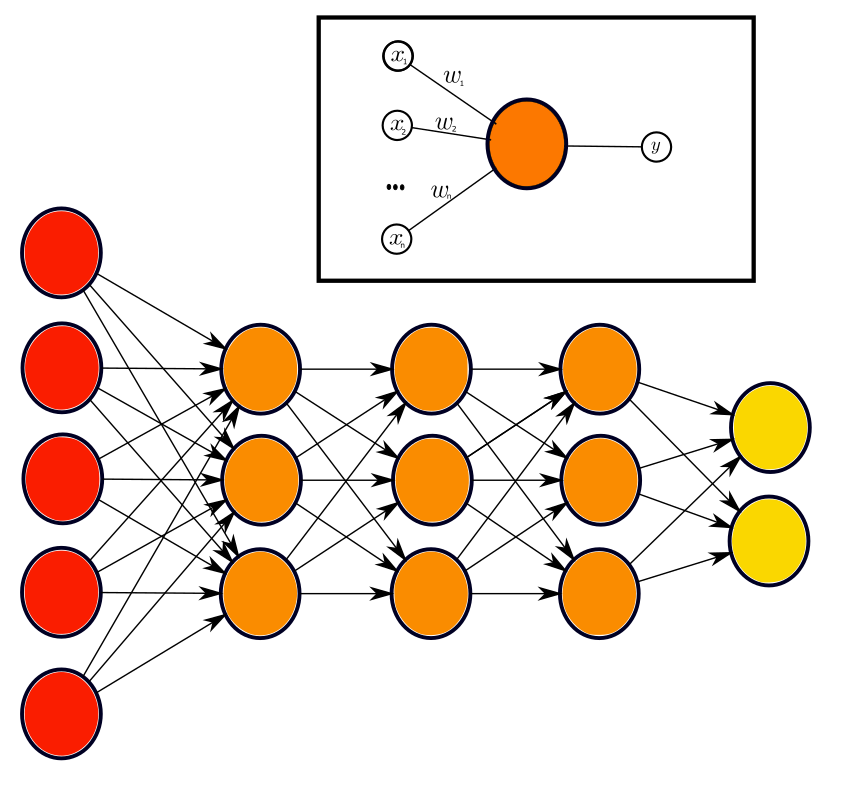
\includegraphics[width=0.8\textwidth]{pic/perceptron.png}
                \caption{Простая схема многослойного перцептрона}
                \label{fig:img2}
            \end{figure}

            \begin{figure}[H]
                \centering
                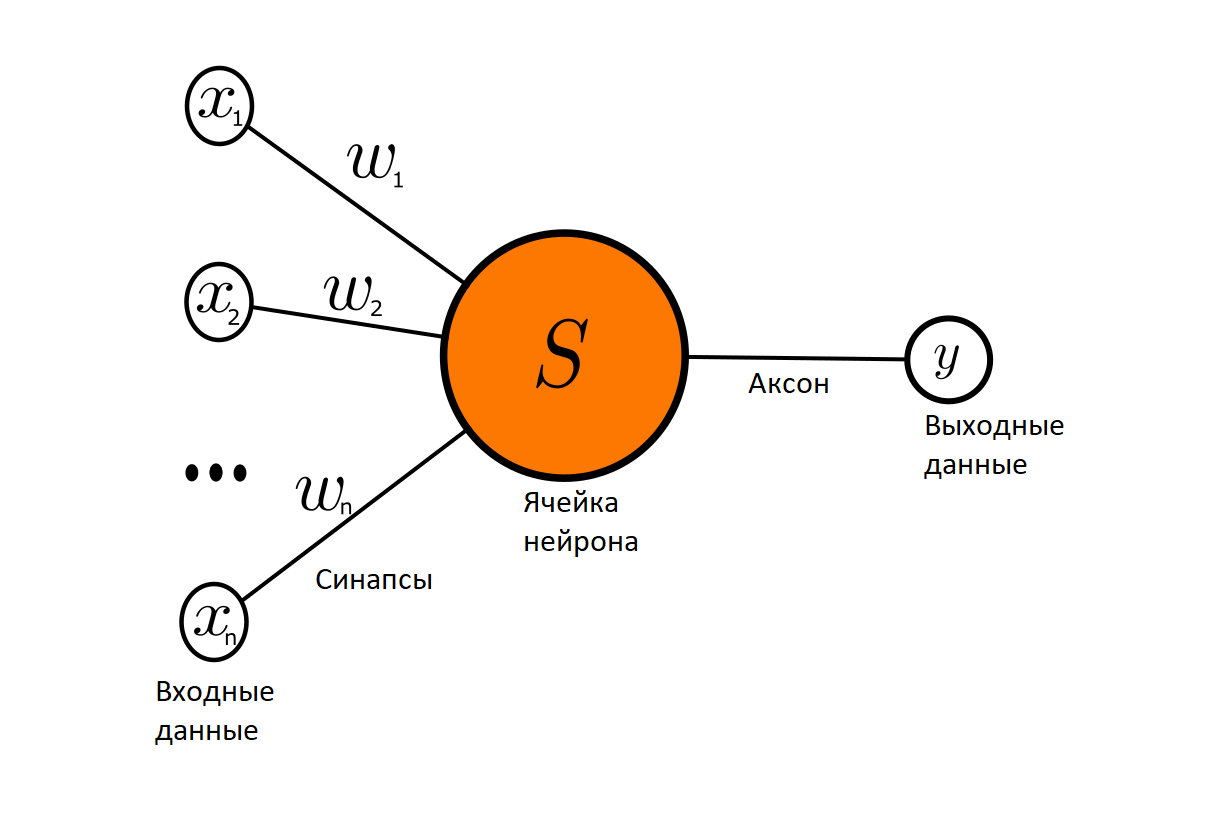
\includegraphics[width=0.9\textwidth]{pic/neuron.png}
                \caption{Устройство нейрона}
                \label{fig:img3}
            \end{figure}

            На рис. 1 изображен многослойный перцептрон, состоящий из искусственных нейронов, соединенных друг с другом синапсом (дугой). На рис. 2 представлен нейрон \cite{neur}, соединяемый с входными данными (это могут быть как исходные данные, так и выходные данные из других нейронов) с помощью синапсов. Каждый синапс имеет собственный вес, определяющий влияние входных данных нейрона на его состояние, а также на значение, которое будет сформировано нейроном как выходные данные, возвращаемые с помощью аксона.
            Состояние нейрона, являющееся содержимым ячейки, определяется выражением \cite{math}

            \[S = \sum_{i = 1}^n x_i w_i , \eqno(1)\]

            где $n$ "--- число синапсов нейрона;
                $w_i$ "--- вес i-того синапса;
                $x_i$ "--- значение i-го входа нейрона.

            Выходные данные, передаваемые через аксон, вычисляются по формуле

            \[y = f (S), \eqno(2)\]

            где $y$ "--- выходные данные;
                $S$ "--- выражение состояния нейрона;
                $f$ "--- активационная функция, вид которой определяется в зависимости от поставленной задачи \cite{Neuron}.

            % Пусть нейрон преобразует один входной элемент в один выходной элемент в некоторый дискретный момент времени с шагом $\tau$. Например, пусть входной сигнал "--- $x$, а $\alpha$ "--- характеристика (или их набор) рассматриваемого нейрона $f(x, \alpha)$.
            % \begin{enumerate}
            %     \item Пороговый нейрон (где $x \geq 0$ и $\alpha > 0$)
            %         \begin{equation*}
            %             f(x) = 
            %             \begin{cases}
            %             0 &\text{если $x < \alpha$}\\
            %             1 &\text{если $x \geq \alpha$}
            %             \end{cases}
            %         \end{equation*}    
            %     \item (при $-\infty < x < \infty, \alpha > 0$) \[f(x) = \frac{x}{\alpha + | x |}\]
            %     \item (при $-\infty < x < \infty, \alpha > 0$) \[f(x) = th\frac{x}{\alpha}\]
            %     \item Многопараметрические нейроны: (при $\alpha_2 > 0, \hspace{5pt} -\infty < x, \hspace{5pt} \alpha_{1, 3} < \infty$)
            %         \[f(x) = \frac{\alpha_1 \cdot x + | x | \cdot x}{\alpha_2 + \alpha_3 \cdot | x | + x^2}\]
            %     \item (при $\alpha_3 > 0, \hspace{5pt} -\infty < x, \hspace{5pt} \alpha_{1, 2, 4, 5} < \infty$)
            %         \[f(x) = \frac{\alpha_1 \cdot x + \alpha_2 \cdot x^2 + x^3}{\alpha_3 + \alpha_4 \cdot | x | + \alpha_5 \cdot x^2 + | x |^3}\]
            % \end{enumerate}

    \subsection{Сверточная нейронная сеть}

        В частности, для обнаружения объектов на изображении, может использоваться сверточная нейронная сеть "--- специальная разновидность нейронной сети, предложенная Яном Лекуном, обрабатывающая данные с сеточной топологией и характеризующая технологию компьютерного зрения. Название этой сети напрямую связано с алгебраической линейной операцией свертки, сутью которой является получение функции из двух других функций. Сверточная сеть предполагает использование операции свертки вместо общей операции умножения на матрицу в по крайней мере одном слое.

        \begin{figure}[H]
            \centering
            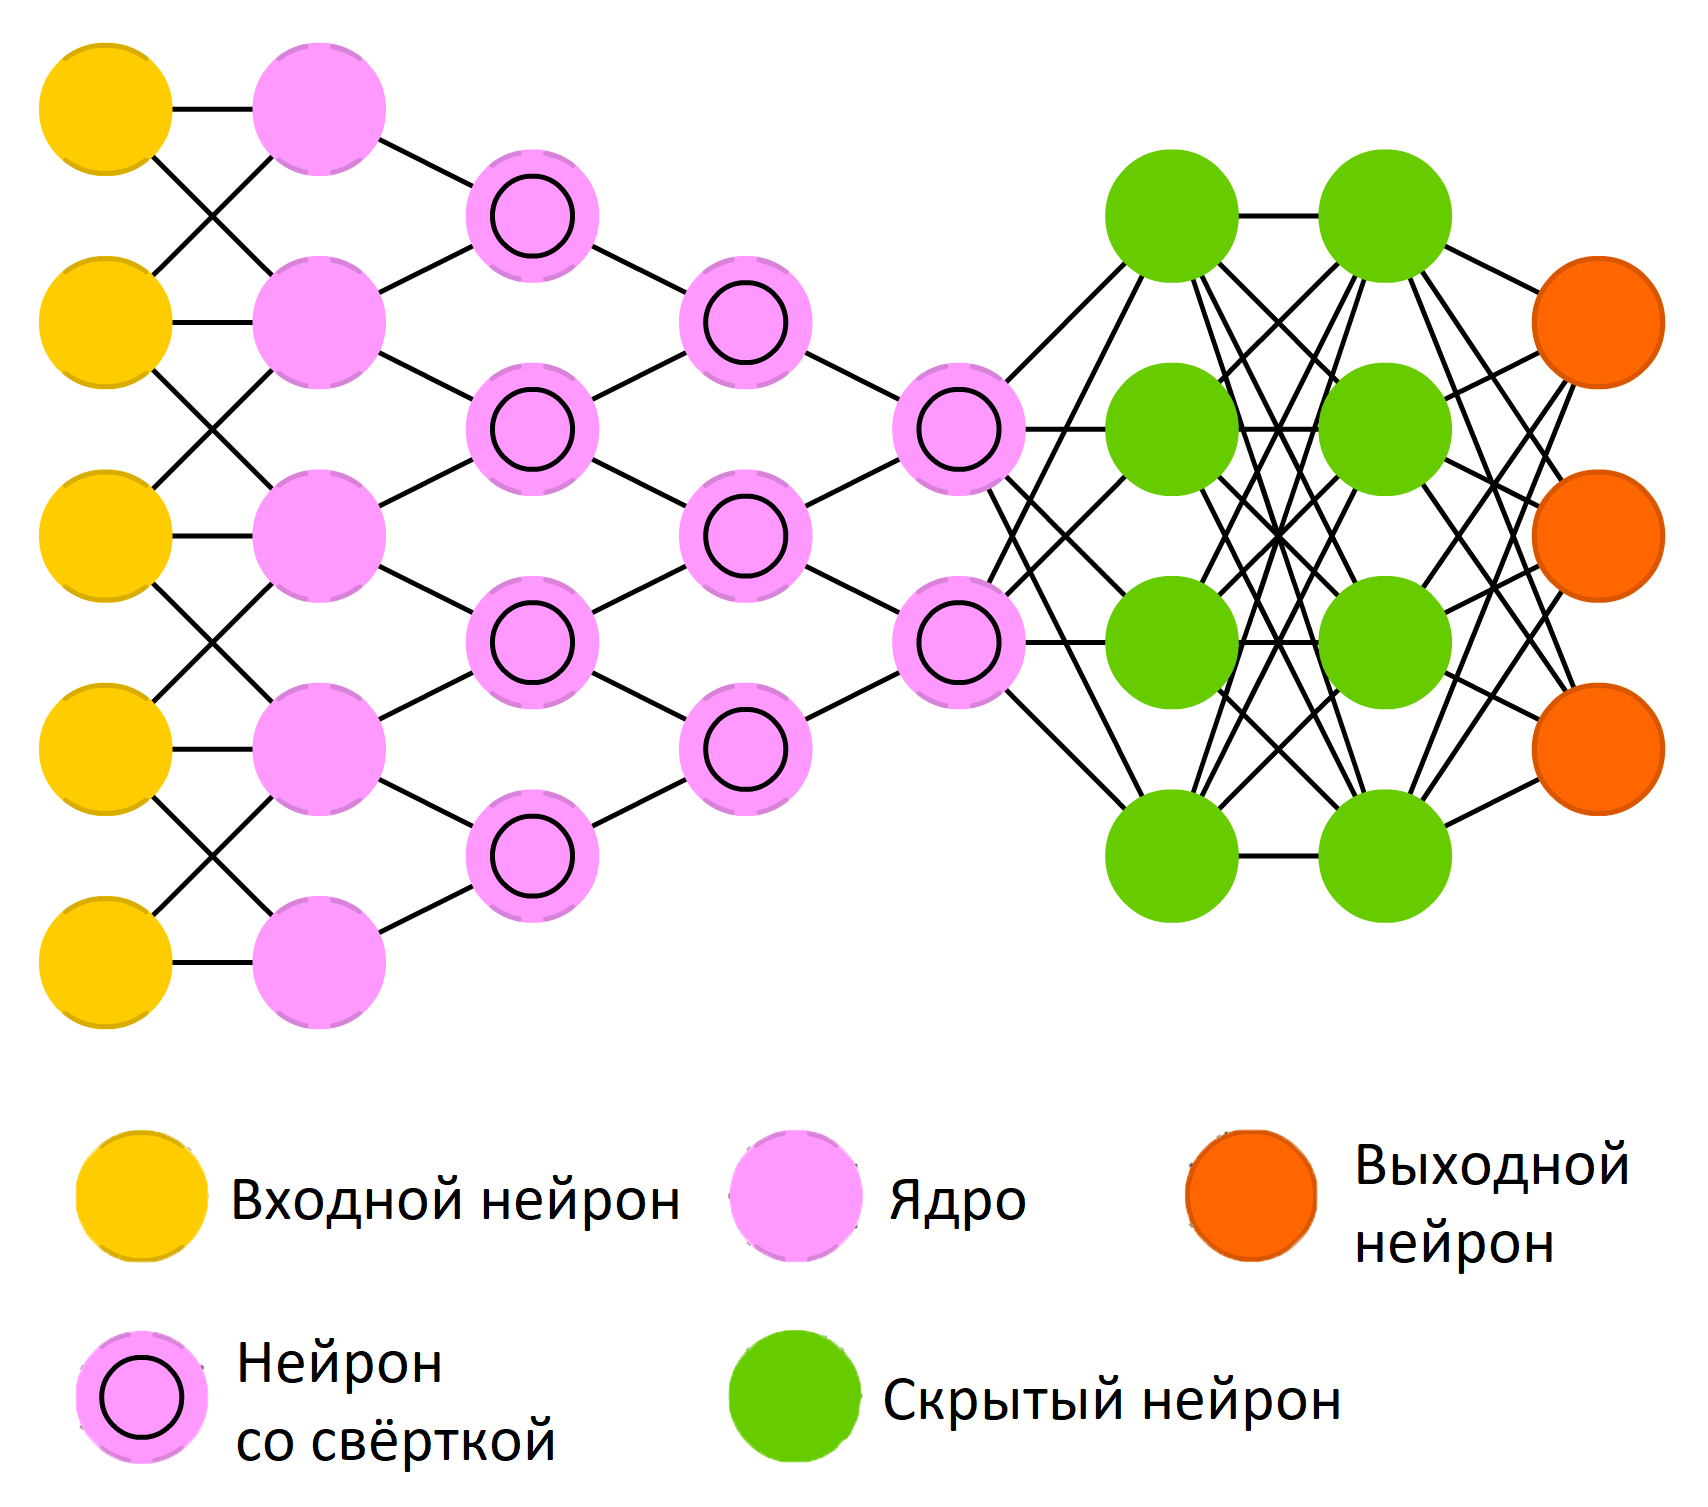
\includegraphics[width=0.6\textwidth]{pic/cnn.png}
            \caption{Схема сверточной нейросети}
            \label{fig:img4}
        \end{figure}

        \subsubsection{Двумерная сверточная нейронная сеть}
            
            В данной нейросети используется операция двумерной свертки. Определим ядро как матрицу весов. Оно перемещается над двумерным изображением, поэлементно совершая операцию умножения с той частью входных данных, над которой оно находится в текущий момент времени, после чего суммирует все полученные значения в один выходной пиксель (см рисунок 4).

            Ядро выполняет этот алгоритм каждый раз при перемещении, таким образом преобразуя двумерную матрицу в матрицу признаков. Признаки на выходе являются взвешенными суммами (веса определяются значениями ядра) входных признаков, находящихся в том же месте, что и выходной пиксель на входном слое.

            \begin{figure}[H]
                \centering
                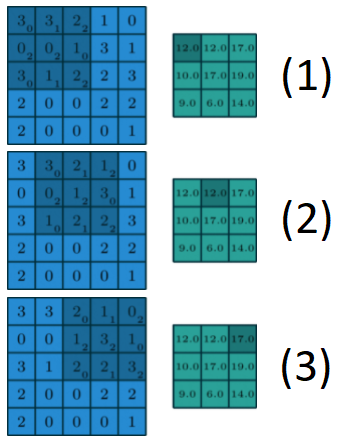
\includegraphics[width=0.5\textwidth]{pic/svertka.png}
                \caption{Операция двумерной свертки на примере трех шагов}
                \label{fig:img8}
            \end{figure}

            Входной признак определяется по тому, находится ли он в зоне создающего выходные данные ядра, или нет. Вследствие этого, размер ядра сверточной нейросети определяет количество признаков, которые будут объединены с целью получения нового признака на выходе \cite{Network}.

            В примере на рисунке 4 будет 25 признаков на входе и 9 признаков на выходе. При использовании стандартного слоя необходимо было бы работать с 225 параметрами, а каждый выходной признак был бы взвешенной суммой всех входных признаков. Благодаря свертке можно получить аналогичный результат с 9 параметрами, так как каждый выходной признак является результатом только одного входного.

            Таким образом, ранее описанную формальным языком операцию свертки для изображения, определяемого одним каналом, можно определить следующим выражением \cite{Svertka}:

            \[y_{i, j} = \sum^S_{n = 1} \sum^S_{m = 1} w_{n, m} x_{((i - 1)+n, (j - 1)+m)}, \eqno(3)\]

            где $w_{i, j}$ "--- значение элемента ядра свертки на позиции $(i, j)$;\\
                $y_{i, j}$ "--- значение пикселя выходного изображения на позиции $(i, j)$;\\
                $x_{((i - 1)+n, (j - 1)+m)}$ "--- значение пикселя входного изображения на позиции\\ $((i - 1)+n, (j - 1)+m)$;\\
                $S$ "--- размерность ядра свертки.

        \subsubsection{Многоканальная версия сверточной нейронной сети}

            На практике чаще всего входное изображение состоит из 3 каналов, число которых постепенно увеличивается с глубиной сети.

            Количество ядер соответствует количеству входных каналов, причем каждое из ядер является уникальным и определяет свой канал. Совокупность ядер является фильтром, и каждый фильтр в сверточном слое нейросети (сверточный слой "--- тот, в котором нейроны применяют операцию свертки) создает только один выходной канал по следующему алгоритму: каждое из ядер перемещается по соответствующему ему входному каналу и при этом создает его измененную версию. Веса ядер могут быть различны в зависимости от того, над каким входным каналом необходимо осуществить больше операций (например, фильтр может задавать ядру зеленого канала больший вес, чем другим каналам, для того чтобы лучше обращать внимание на различия в образах, состоящих из зеленого канала).

            \begin{figure}[H]
                \centering
                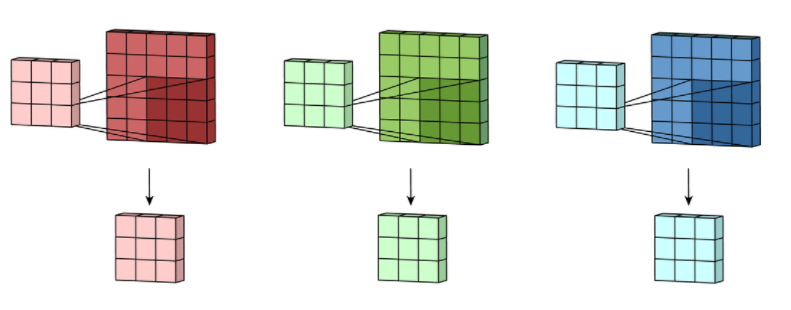
\includegraphics[width=0.6\textwidth]{pic/rgb.png}
                \caption{Свертка при трех входных каналах}
                \label{fig:img5}
            \end{figure}

            После получения всех измененных версий входных каналов осуществляется их суммирование для формирования одного канала. Ядро каждого из каналов определяет одну версию конкретного канала, и фильтр создает один общий выходной канал на их основе.

            \begin{figure}[H]
                \centering
                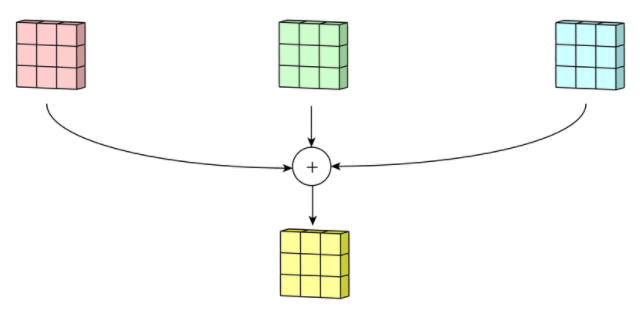
\includegraphics[width=0.6\textwidth]{pic/tino.png}
                \caption{Генерация одного выходного канала}
                \label{fig:img6}
            \end{figure}

            Каждый выходной файл имеет свое смещение. Для получения конечного выходного канала необходимо добавить смещение к каждому выходному каналу:

            \begin{figure}[H]
                \centering
                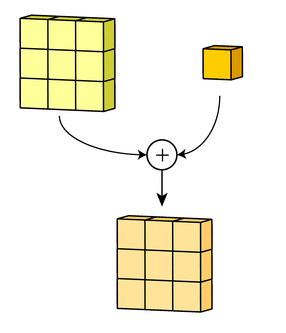
\includegraphics[width=0.3\textwidth]{pic/cvc.png}
                \caption{Формирование конечного выходного канала}
                \label{fig:img7}
            \end{figure}

            При любом количестве фильтров результат не меняется: вход обрабатывается каждым фильтром с помощью своего уникального набора ядер и скалярного смещения по представленному ранее алгоритму, и результатом процесса является один выходной канал для одного фильтра. При том, что число выходных каналов соответствует числу фильтров, следующим шагом полученные выходные каналы суммируются, чтобы составить общий выход \cite{Network}.

    \subsection{Метод обратного распространения ошибки}

        Метод обратного распространения ошибки (Backpropagation) является одним из эффективных средств улучшения обучения нейросети и способствующий более продуктивному поиску закономерностей, прогнозированию и качественному анализу. Сети, которые используют этот метод, называются сетями обратного распространения. Смысл их названия заключается в том, что алгоритм их обучения подразумевает распространение ошибки от выходного слоя к входному, то есть по направлению, противоположному направлению распространения сигнала при естественном функционировании сети \cite{mathapp}.

        Нейросеть обратного распространения является полносвязной, то есть синапсы между нейронами присутствуют в оба направления сети.

        Основной задачей обыкновенного обучения нейросети является определение функции активации, которая в общем случае имеет бесконечное множество решений при ограниченном наборе входных данных. При реализации сети с обратным распространением необходимо ограничить пространство поиска, и для этого ставится задача минимизации целевой функции ошибки нейросети, которая находится с помощью следующей формулы, называемой методом наименьших квадратов:

        \[E(w) = \frac{1}{2} \sum^n_{i = 1} (y_i - d_i)^2, \eqno(4)\]
        где $y_i$ "--- значение i-ого выходного нейрона;
            $d_i$ "--- целевое значение i-го выхода;
            $n$ "--- количество нейронов в выходном слое.
        
        Основным алгоритмом обучения нейросети является использование градиентного спуска, в котором на каждой итерации (шаге обучения) происходит изменение веса нейрона следующим образом:

        \[\Delta w_{ij} = - \eta \cdot \frac{\partial E}{\partial w_{ij}}, \eqno(5)\] где $\eta$ "--- параметр, который определяет скорость процесса обучения.
        В свою очередь, \[\frac{\partial E}{\partial w_{ij}} = \frac{\partial E}{\partial y_{i}} \cdot \frac{\partial y_i}{\partial S_{j}} \cdot \frac{\partial S_j}{\partial w_{ij}}, \eqno(6)\]
        где $y_i$ "--- значение i-ого выходного нейрона;
            $S_j$ "--- взвешенная сумма входных сигналов, вычисляемая по формуле $(1)$.

        Стоит отметить, что в равенстве $(6)$ третий множитель можно определить как \[\frac{\partial S_j}{\partial w_{ij}} = x_i, \eqno(7) \]
        где $x_i$ "--- значение i-ого входного нейрона.

        Первый же множитель можно выразить следующим образом:
        \[\frac{\partial E}{\partial y_i} = \sum_k \frac{\partial E}{\partial y_k} \cdot \frac{\partial y_k}{\partial S_k} \cdot \frac{\partial S_k}{\partial y_i} = \sum_k \frac{\partial E}{\partial y_k} \cdot \frac{\partial y_k}{\partial S_k} \cdot w^{(n)}_{jk}, \eqno(8) \]
        где $k$ "--- число нейронов в n-ом слое.

        Стоит ввести вспомогательную переменную, благодаря которой можно определить рекурсивную формулу для определения (n-1)-го слоя:

        \[\delta^{(n-1)}_j = \frac{\partial E}{\partial y_j} \cdot \frac{\partial y_j}{\partial S_j}, \eqno(9)\]

        Если известно состояние n-го слоя, тогда рекурсивная формула будет иметь вид:

        \[\delta^{(n-1)}_j = \left[\sum_k \delta_k^{(n)} \cdot w_{jk}^{(n)} \right] \cdot \frac{\partial y_j}{\partial S_j}, \eqno(10) \]

        Поскольку известен целевой вектор, состоящий из значений, которые должны быть получены сетью в результате работы над данным набором входных значений, можно определить последний слой нейросети:

        \[\delta_j^{(N)} = (y_i^{(N)} - d_i) \cdot \frac{\partial y_j}{\partial S_j}, \eqno(11)\]

        где $N$ "--- номер последнего слоя сети.

        Теперь, имея все необходимые переменные и выражения, можно записать выражение метода градиентного спуска в раскрытом виде:

        \[\Delta w_{ij}^{(n)} = - \eta \cdot \delta_j^{(n)} \cdot x_i^n, \eqno(12) \]

        Учитывая все изложенные ранее формулы и определения \cite{math}, получается полный алгоритм обучения нейросети обратного распространения:

        \begin{enumerate}
            \item Подача на вход нейронной сети один из требуемых образов и определение значений выходных нейронов.
            \item Определение выходного слоя сети с помощью формулы $(11)$ и расчет изменений весов выходных нейронов по формуле $(12)$.
            \item Применить рекурсивную формулу $(10)$ и $(12)$ соответственно, а также рассчитать $\Delta w_{ij}^{(n)}$ для всех остальных слоев сети, то есть $n = N - 1, \cdots, 1$.
            \item Скорректировать все веса нейросети по формуле:
            \[w^{(n)}_{ij} (t) = w^{(n)}_{ij} (t - 1) + \Delta w^{(n)}_{ij} (t). \eqno(13)\]
            \item Если ошибка существенна, осуществить переход к шагу 1.
        \end{enumerate}


    \subsection{Роль глубокого обучения}

        Большая часть задач искусственного интеллекта решается в два этапа: корректный подбор признаков, а затем их передача алгоритму машинного обучения. В качестве примера можно взять задачу идентификации объекта по звуку речи. В ней полезным признаком является речевой тракт или же голосовой диапазон. Он
        позволяет с большой точностью определить, является ли говорящий объект мужчиной, женщиной или
        ребенком.
        Но далеко не во всех задачах можно сразу понять, какие признаки стоит выделять: для этого достаточно рассмотреть ситуацию, в которой необходимо написать программу обнаружения автомобилей на фотографиях. Известно, что у автомобилей есть колеса, вследствие чего можно в качестве одного из признаков выбрать наличие колеса. Однако нельзя сказать, что описание колеса на уровне пикселей легкая задача.
        Колесо характеризуется простой геометрической формой, но его распознавание на изображении
        нередко бывает осложнено различными факторами, такими как отбрасывание теней, наличие щитка для защиты колеса от грязи, объекты на переднем плане, которые могут закрывать часть колеса, и т. д.

        В качестве решений подобной задачи рассматривают использование машинного обучения не только как способа нахождения отображения представления на результат, но и для определения самого представления, то есть, подразумевается использование глубокого обучения. С помощью представлений, которые являются результатом обучения, удается более точно определить объект на изображении, чем с помощью представлений, созданных вручную. В качестве характерного преимущества подобных реализаций стоит отметить быструю адаптацию ИИ к новым задачам с учетом минимального вмешательства человека в изменение структуры конкретной нейронной сети \cite{Gud}.

    \subsection{Компоненты глубокого обучения}

        Важную роль в алгоритме обучения представлений является понятие автокодировщика. Обучение автокодировщиков устроено таким образом, что при каждой последующей итерации, в ходе которой происходит кодирование и декодирование некоторой информации, каждое новое представление характеризуется всё большим количеством полезных свойств при наименьшей потери обрабатываемой информации.

        Сутью моделирования алгоритма обучения признаков или же самого признака является получение различных факторов вариативности. Например, в случае анализа изображения машины такие абстракции как её положение, цвет, яркость солнца и его высота над горизонтом являются факторами вариативности, а в случае анализа изображения лица человека факторами вариативности будут являться его цвет, положение и цвет глаз, их расстояние друг от друга, положение и форма губ, и так далее. Однако большое количество факторов вариативности, получаемых в ходе проектирования признаков или иным способом, следует отбросить в силу их влияния на все данные, доступные анализу в процессе обучения нейронной сети (например, форма губ человека при изучении изображения лица зависит от угла зрения и может быть распознана алгоритмом машинного обучения некорректно) \cite{Gud2}.

    \subsection{Устройство модели глубокого обучения}

        Определение объекта на изображении, представленном в виде набора значений пикселей, трудно решаема при использовании функции отображения множества пикселей в распознаваемый объект. Использование в рассматриваемом случае глубокого обучения на порядок упрощает задачу за счёт разбиения исходного набора пикселей на некоторое количество более простых вложенных отображений, описываемых отдельным слоем модели для каждого. Входные данные в виде изображения представляют собой входной слой. После видимого слоя идет совокупность скрытых слоев, представляющих из себя слои математических функций, каждый из которых предназначен для вычисления значения, являющегося специфичным для ожидаемого результата (их количество напрямую определяет глубину обучения, так как каждый из них извлекает из анализируемого изображения некоторые признаки, и чем больше таких слоев, тем более абстрактные признаки будут получены из исходных данных). Модель самостоятельно определяет пользу каждой из абстракций при конструировании связей в наблюдаемых данных. Завершающим глубокое обучение и определяющим (в данном случае) объект на изображении является выходной слой. На рисунке 8 в составе модели глубокого обучения представлены 3 скрытых слоя, а также слой входных данных и слой выходных данных. При анализе изображения, в силу доступности информации об исходных пикселях (определяемых входным слоем), первый скрытый слой определяет границы совокупностей пикселей с помощью сравнения последних по признаку яркости соседних пикселей. Имея характеристики границ множеств пикселей, полученные в результате действия первого скрытого слоя, второй определяет углы и контуры, представляемые в виде набора границ. На основании этих данных третий скрытый слой осуществляет распознавание частей конкретных объектов на изображении, представленных в виде совокупностей углов и контуров отдельного вида. А последний, выходной слой определяет объекты на изображении по информации о частях этих объектов \cite{Gud}.

        \begin{figure}[H]
            \centering
            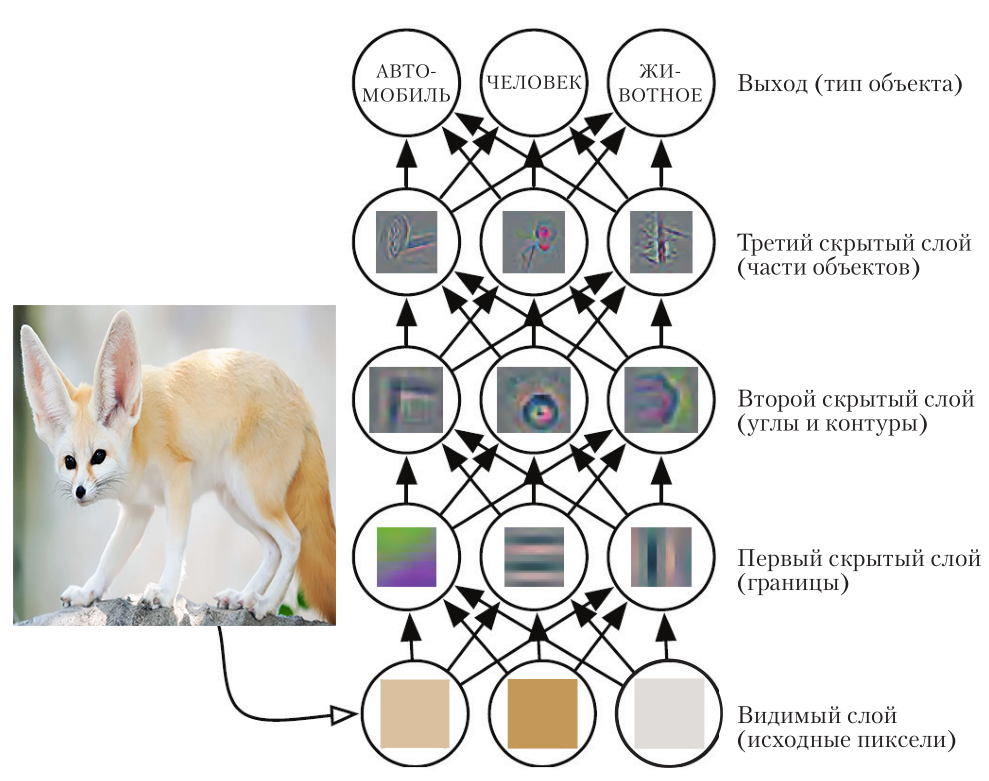
\includegraphics[width=0.9\textwidth]{pic/1.png}
            \caption{Пример модели глубокого обучения "--- определение объекта на изображении}
            \label{fig:img1}
        \end{figure}

        
\section{Применение технологии}

    Распознавание визуальных образов является одной из самых важных
    деталей большинства систем управления и анализа информации, а также
    автоматизированных систем. Задачи, которые связаны с определением предметов,
    описываемых конечным перечнем особых свойств и признаков, имеют место в некоторых 
    отраслях деятельности машинного обучения, такие как робототехника, мониторинг, анализ
    визуальных данных, исследования искусственного интеллекта и т.д. Обработка алгоритмами и
    классификация изображений активно используются в кибербезопасности, в системах контроля и
    управления доступом, в системах видеонаблюдения, виртуальной и дополненной
    реальности и информационных поисковых системах. В настоящий момент в
    производстве активно применяются алгоритмы распознавания рукописного текста,
    номеров транспортных средств, отпечатков пальцев, человеческих лиц или иных средств аутентификации человека, имеющие огромный спрос при реализации интерфейсов программ, систем безопасности и иных прикладных целей.

    \subsection{Задачи мониторинга}

        В качестве примера применения искусственных нейронных сетей, выполняющих обнаружение объектов на изображении в целях мониторинга, можно привести задачу определения разнообразных видов и моделей самолётов, которые находятся на территории аэропорта. Результат работы над конкретной проблемой будет представлять из себя информацию, используемую в различных задачах мониторинга взлётно-посадочных полос (например, определение количества самолетов конкретного вида).\\
        Для выполнения этого задания была использована сверточная нейронная сеть, состоящая из пар слоев "--- слоев подвыборки и слоев свертки, каждый из которых в свою очередь состоит из карт признаков. Все карты признаков фильтруют изображение, обнаруживая какой-то один определенный, специфичный для конкретной карты, признак \cite{Svertka}. Количество слоев в рассматриваемой нейросети составило 13. Обучение происходило на выборке, определяющейся четырьмя классами объектов: дороги, растительность, городские сооружения и самолеты. Общее количество образцов изображений для обучающей выборки составило приблизительно 5000.\\
        В связи с тем, что анализ изображения происходит с перекрытием (то есть каждый пиксель изображения анализируется совместно со своими соседними пикселями), повышается способность поиска нужного объекта. Однако при этом появляется возможность многократного вхождения одного и того же объекта сразу в несколько фрагментов. Такой результат работы нейронной сети сложен для обработки, поэтому необходимо применение алгоритма слияния прямоугольников, содержащих объекты.\\
        Нейронная сеть после обработки изображения на выходе совместно с координатными прямоугольниками дает соответствующую каждому из прямоугольников вероятность. Этой вероятностью определяется возможность нахождения координатного прямоугольника над искомым объектом, она определяется числом с плавающей точкой в интервале от 0 до 1. Используемый алгоритм принимает на вход пару, состоящую из координатного прямоугольника и вероятности. Алгоритм слияния состоит из нескольких этапов: создание подсписков из основного списка координатных прямоугольников, фильтрация координатных прямоугольников по вероятности и создание общего координатного прямоугольника \cite{aero}. \\
        Таким образом, в качестве результата деятельности нейронной сети совместно с алгоритмом слияния удалось решить задачу обнаружения самолета на изображении в целях мониторинга.

        \begin{figure}[H]
            \centering
            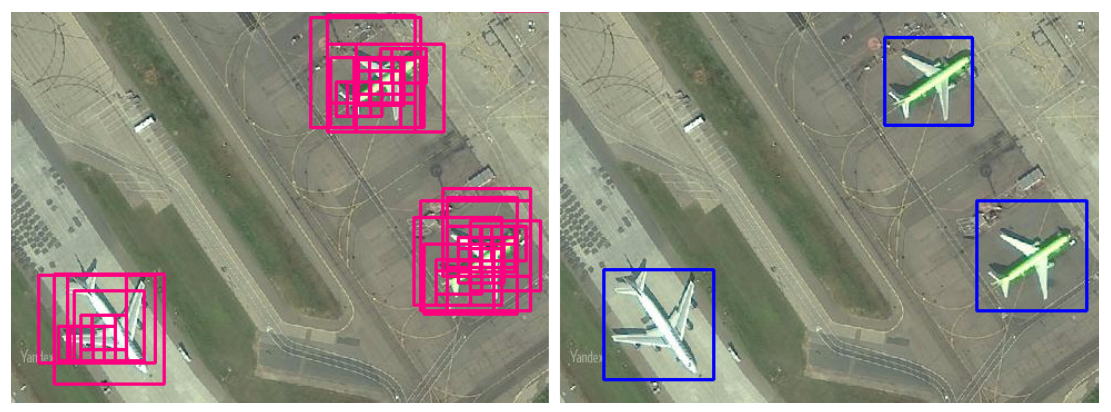
\includegraphics[width=0.9\textwidth]{pic/aero.png}
            \caption{Выделенные объекты интереса до (слева) и после (справа) применения алгоритма слияния}
            \label{fig:img9}
        \end{figure}
        
    \subsection{Задачи анализа визуальных данных}
        Одним из примеров решения задачи анализа визуальных данных методом обнаружения объекта на изображении с помощью нейросети является развивающаяся технология беспилотного управления автомобилем. \cite{automl}\\
        Реализация беспилотных автомобилей состоит из 4 основных пунктов, в каждом из которых глубокое обучение применяется определенным образом:
        \begin{enumerate}
            \item Восприятие (Perception), то есть целью является анализ окружающей среди и обнаружение различных предметов вокруг точки наблюдения;
            \item Локализация (Localization), означающая определение расположения точки наблюдения относительно мира с точностью до 1-3 сантиметров;
            \item Планирование (Planning), при котором, используя восприятие и локализацию, вычисляется траектория от точки A до точки B;
            \item Управление (Control), сутью которого является использование полученной в предыдущем пункте траектории для создания угла поворота и определения значения ускорения.
        \end{enumerate}

        \subsubsection{Восприятие}
            Для того, чтобы изучать окружающую среду, необходимо считывать информацию о ней. Это осуществляется с помощью трех видов сенсоров:
            \begin{enumerate}
                \item Камера;
                \item Лидар (LiDAR, Light Detection and Ranging);
                \item Радар (RADAR, Radio Detection and Ranging).
            \end{enumerate}
            После получения информации, чтобы удостовериться в её надежности, необходимо совершить слияние данных с сенсоров (Sensor Fusion) и проверить, определяют ли собранные материалы в области наблюдения одни и те же объекты. Слияние происходит только между сведениями, полученными двумя разными путями, например с радара и лидара.

        \subsubsection{Локализация}
            В зависимости от выбора алгоритма, различают несколько способов определения местоположения наблюдателя:
            \begin{enumerate}
                \item С помощью знания карты местности и исходного положения до начала движения;
                \item Только с помощью знания карты местности;
                \item При отсутствие знания карты местности и исходного положения;
            \end{enumerate}
            Первые две ситуации используют алгоритм обнаружения ориентира (Landmark Detection), так как метод состоит в обнаружении известных объектов и того, что изображено на карте. Идея последней ситуации состоит в том, чтобы использовать датчики, такие как камеры или стереокамеры, для воссоздания окружающей среды и, следовательно, карты.
    
        \subsubsection{Планирование}
            Планирование происходит в три этапа:
            \begin{enumerate}
                \item Высокоуровневое (глобальное) планирование "--- вычисление маршрута от точки A до точки B;
                \item Поведенческое планирование "--- прогнозирование того, что будут делать окружающие объекты, и принятие решений в зависимости от этого;
                \item Путевое (локальное) планирование "--- создание траектории с учетом обхода объектов, являющихся препятствиями.
            \end{enumerate}

        \subsubsection{Управление}
            Так как управлением является процесс вычисления угла поворота и ускорения на основе данных полученных в ходе планирования, использование глубокого обучения на данном этапе является предпочтительным.
        
        \subsubsection{Итоги}
            Таким образом, обнаружение объектов на изображении весомо способствует реализации работы беспилотных автомобилей на этапах восприятия, локализации и планировании, выполняя при этом задачу анализа визуальных данных.\\
            % Компьютерное зрение, которое используется в беспилотном автомобиле, можно реализовать с помощью только камер и радаров. Особенность такого метода заключается в локальном использовании техники: в бортовой компьютер загружаются базовые карты, которые затем обрабатываются нейросетями, после чего сравнивают реальность с загруженными картами. Стоит отметить, что транспорт будет плохо ориентироваться в городах, подобных Лондону, в связи с повышенной там частотой природных явлений, которые затрудняют восприятие окружающей среды даже человеку. Кроме того, машина будет активно переобучаться в городах, подобных Москве, где всё активно строится и ремонтируется \cite{auto}.
            \begin{figure}[H]
                \centering
                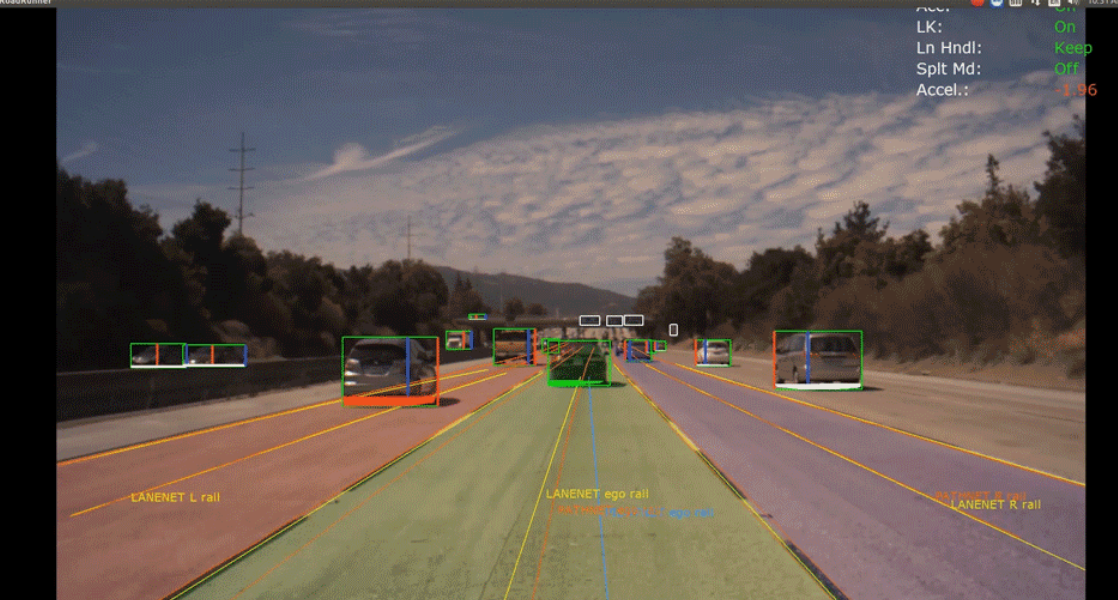
\includegraphics[width=0.9\textwidth]{pic/auto.png}
                \caption{Использование обнаружения объекта на изображении в беспилотном автомобиле на этапе восприятия}
                \label{fig:img20}
            \end{figure}

\conclusion

    В данной работе были рассмотрены следующие темы:
    \begin{enumerate}
        \item Основополагающая теоретическая информация об устройстве нейронной сети и сверточной нейронной сети в частности;
        \item Алгоритм свертки для одного или нескольких каналов изображения;
        \item Метод обратного распространения ошибки вместе с выводом его пошагового алгоритма со всеми нужными для этого формулами;
        \item Важность роли глубокого обучения как средства, позволяющего использовать нейронную сеть для обнаружения объекта на изображении, а также его логика и компоненты.
    \end{enumerate}
    
    Также были приведены примеры задач, в которых использование технологии обнаружения объекта на изображении является лучшим решением, в частности, были рассмотрены задачи мониторинга и анализа визуальных данных.

    В качестве заключения можно также добавить, что суть нейросетей определяется совокупностью понятий математического анализа, теории вероятностей, линейной алгебры и теории графов. В современности есть множество примеров, в которых применяются методы обнаружения объектов на изображении с помощью нейронных сетей, и с каждым годом их количество будет только расти.

\begin{thebibliography}{99}
    \bibitem{neur} Короткий С., ''Нейронные сети: Основные положения'', [Электронный ресурс] : [статья] / URL: http://www.shestopaloff.ca/kyriako/Russian/Artificial_Intelligence/Some_publications/Korotky_Neuron_network_Lectures.pdf  (дата обращения 27.04.2021) Загл. с экрана. Яз. рус.
    \bibitem{math} Короткий С., ''Нейронные сети: Алгоритм обратного распространения'', [Электронный ресурс] : [статья] / URL: http://masters.donntu.org/2009/fvti/trubarov/library/article2.htm (дата обращения 27.04.2021) Загл. с экрана. Яз. рус.
    \bibitem{Neuron} Baestaens D. E., Van Den Bergh W. M., Wood D., ''Neural Network Solution for Trading in Financial Markets'', Pitman publishing, 1994 г., Яз. англ.
    \bibitem{Network} Исаков С., ''Как работает сверточная нейронная сеть: архитектура, примеры, особенности'', [Электронный ресурс] : [статья] / URL: https://neurohive.io/ru/osnovy-data-science/glubokaya-svertochnaja-nejronnaja-set/ (дата обращения 27.04.2021) Загл. с экрана. Яз. рус.
    \bibitem{Svertka} Дорогой Я., ''Архитектура обобщенных сверточных нейронных сетей'', [Электронный ресурс] : [статья] / URL: http://www.it-visnyk.kpi.ua/wp-content/uploads/2012/08/54_36.pdf (дата обращения 27.04.2021) Загл. с экрана. Яз. рус.
    \bibitem{mathapp} Стариков А., ''Нейронные сети — математический аппарат'', [Электронный ресурс] : [сайт] / URL: https://basegroup.ru/community/articles/math (дата обращения 27.04.2021) Загл. с экрана. Яз. рус.
    \bibitem{Gud} Гудфеллоу Я., Бенджио И., Курвилль А., ''Глубокое обучение'', г. Москва, Издательство ДМК, 2018 г., Яз. рус.
    \bibitem{Gud2} Sutskever I., Martens J., Dahl G., and Hinton G., ''On the importance of initialization and momentum in deep learning.'', ICML, 2013 г., Яз. англ.
    \bibitem{aero} Смирнов А. В., Иванов Е. С., ''Использование механизма сверточных нейронных сетей для поиска объектов на аэрофотоснимках'' [Электронный ресурс] : [статья] / URL: http://psta.psiras.ru/read/psta2017_4_85-99.pdf (дата обращения 10.04.2021) Загл. с экрана. Яз. рус.
    \bibitem{automl} Cohen J., ''Deep Learning in Self-Driving Cars'', [Электронный ресурс] : [статья] / URL: https://becominghuman.ai/deep-learning-algorithms-in-self-driving-cars-14b13a895068 (дата обращения 03.05.2021) Загл. с экрана. Яз. англ.
    % \bibitem{auto} Туренко Е., ''Как работает беспилотный транспорт'', [Электронный ресурс] : [статья] / URL: https://tproger.ru/articles/self-driving-cars-howto/, дата обращения 29.04.2021, Яз. рус.
\end{thebibliography}

\end{document}
